\documentclass[9pt]{beamer}
%\usetheme{CambridgeUS}
\usetheme{Antibes}
\usecolortheme[RGB={120,130,235}]{structure}

\usepackage{graphics}
\usepackage{marvosym}
\usepackage{graphicx}
\usepackage{latexsym}
\usepackage{amsmath}
\usepackage{amsfonts,amssymb}
\usepackage{ mathrsfs }
\usepackage{amsthm}
\usepackage{multimedia}
\usepackage{subcaption}
\usepackage{hyperref}
\usepackage{breqn}
\usepackage{wasysym}
\usepackage{xcolor}
\usepackage{ stmaryrd }
\newtheorem{prop}{Proposition}

%Define New Macros
%\input macros
\renewcommand\o{\omega}
\newcommand{\deriv}{\mbox{d}}
\newcommand{\Real}{\mathbb R}
\newcommand{\T}{\mathbb T}
\newcommand{\norm}[1]{\|#1\|}
\newcommand{\abs}[1]{\left\vert#1\right\vert}
\newcommand{\set}[1]{\left\{#1\right\}}
\newcommand{\subheading}[1]{\noindent \textbf{#1}}
\newcommand{\grad}{\nabla}
\newcommand{\diverg}{\textup{div} }
\newcommand{\jump}[1]{[#1]}
\newcommand{\limit}[2]{\lim_{#1 \rightarrow #2}}
\newcommand{\mollify}[1]{ \mathcal{J}_\epsilon #1 }
\newcommand{\conv}[2]{#1 \ast #2}
\newcommand{\D}{D}
\newcommand{\K}{\mathcal{K}}
\newcommand{\ineqtext}[1]{ ^{\text{\tiny #1}}}
\newcommand{\wknorm}[2]{\norm{#1}_{L^{#2,\infty}}}
%\newcommand{\wknorm}[2]{\abs{#1}_{L_w^{#2}}}
\newcommand{\wkspace}[1]{L^{#1,\infty}}
%\newcommand{\wkspace}[1]{L_w^{#1}}
\newcommand{\F}{\mathcal{F}}
\newcommand{\G}{\mathcal{G}}
\newcommand{\eps}{\epsilon}
\newcommand{\lap}{\Delta}

%Nancy's macros
\newcommand{\reg}[1]{#1^\epsilon}
\newcommand{\Lpr}[1]{L^{#1}(\mathbb{R}^n)}
\newcommand{\Lp}[1]{L^{#1}(\Omega)}
\newcommand{\intreal}{\int_{\mathbb{R}^2}\hspace{-8pt}}
\newcommand{\energy}{\mathcal{F}}
\newcommand{\modenergy}{\mathcal{E}_H}
\newcommand{\kernel}{\mathcal{K}}
\newcommand{\into}{\int_{D}}
\newcommand{\intot}{\int_{D_T}}
\newcommand{\ball}{B_n}
\newcommand{\balltime}{B_n\times [0,T]}

\newcommand{\brak}[1]{\langle #1 \rangle} 
\usepackage{url}
\makeatletter
\g@addto@macro{\UrlBreaks}{\UrlOrds}
\makeatother
\newcommand*{\vpointer}{\vcenter{\hbox{\scalebox{2}{\Huge\pointer}}}}


\DeclareMathOperator{\R}{\mathbb{R}}

\title[Midterm Presentation]{Scientific Computation of Two--Phase Ferrofluid Flows} 
\author[Midterm Presentation]{Gareth Johnson \\[.3cm] Faculty Adviser: Prof. Ricardo Nochetto } 
\institute[] 
{
	University of Maryland\\ 
	AMSC 663: Advanced Scientific Computing I\\ 
	Supported by Johns Hopkins University Applied Physics Lab
}
\date[November 2018]{November 1, 2018}


\begin{document}
\begin{frame}
	\titlepage
\end{frame}

\section{Solving PDEs}
\begin{frame}{Solving PDEs using deal.II}
	Each program in deal.II can be broken down into 5 main steps:
	\begin{itemize}
		\item[1)] Generate the mesh.
		
		\item[2)] Distribute degrees of freedom and set up the matrices for the associated system.
		
		\item[3)] Compute the left and right hand sides of the system. 
		
		\item[4)] Solve the system numerically.
		
		\item[5)] Output the solution in a specific format for visualization or post-processing.
	\end{itemize}
\end{frame}

\section{Examples}
\begin{frame}{Example 1}
	The first PDE solved was Poisson's equation:
	$$
		\begin{cases}
		-\lap u = f(x) &\text{in }\Omega\\
		u = 0 & \text{on }\partial\Omega,
		\end{cases}
	$$
	where $f(x) = 1$ and $\Omega = [0,1]^2$.
	
	\begin{minipage}{.5\paperwidth}
		\centering
		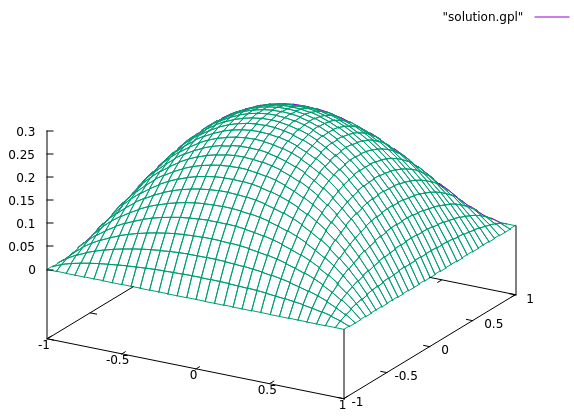
\includegraphics[scale=.39]{Solu1-gnuplot.png}
	\end{minipage}%
	\begin{minipage}{.4\paperwidth}
		\centering
		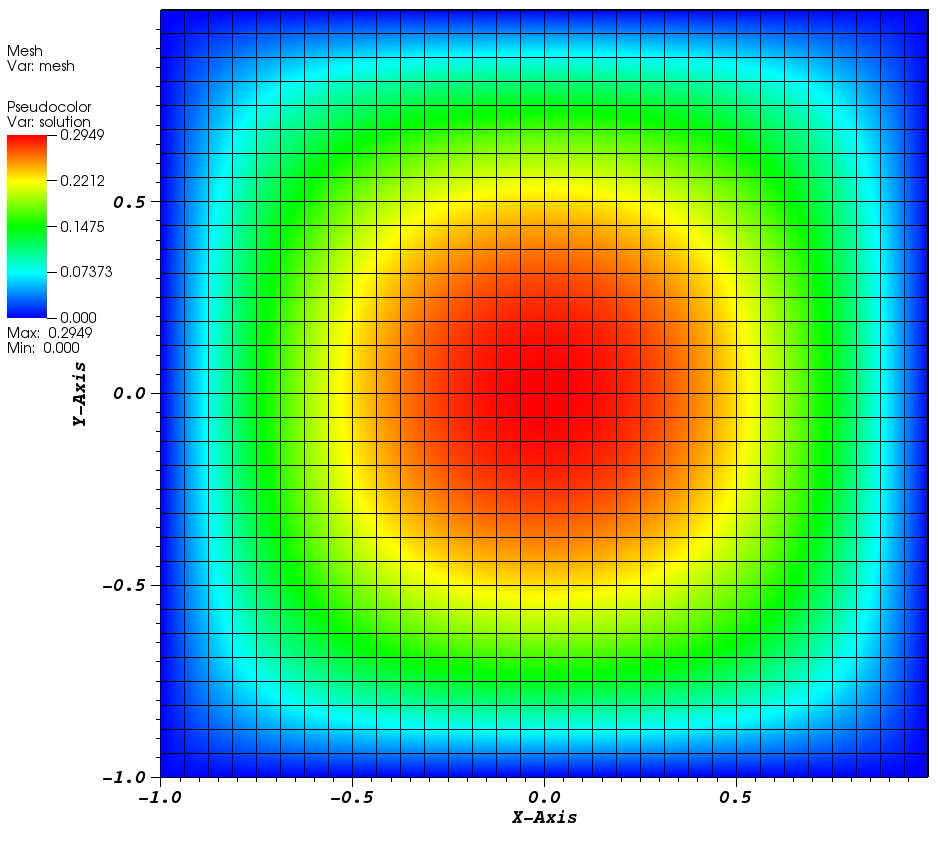
\includegraphics[scale=.7]{Solu1-visit.png}
	\end{minipage}
\end{frame}

\begin{frame}{Example 2}
The second PDE solved was Poisson's equation:
$$
\begin{cases}
-\lap u = f(x) &\text{in }\Omega\\
u = g(x) & \text{on }\partial\Omega,
\end{cases}
$$
where 
$$
	f(x) = \begin{cases}
	4(x^4 + y^4) & \text{if } \Omega \subset \Real^2\\
	4(x^4 + y^4 + z^4) & \text{if } \Omega \subset \Real^3\\
	\end{cases}, \quad 
	g(x) = \begin{cases}
	x^2 + y^2 & \text{if } \Omega \subset \Real^2\\
	x^2 + y^2 + z^2 & \text{if } \Omega \subset \Real^3\\
	\end{cases},
$$ and $\Omega$ is the unit square or cube.


\centering
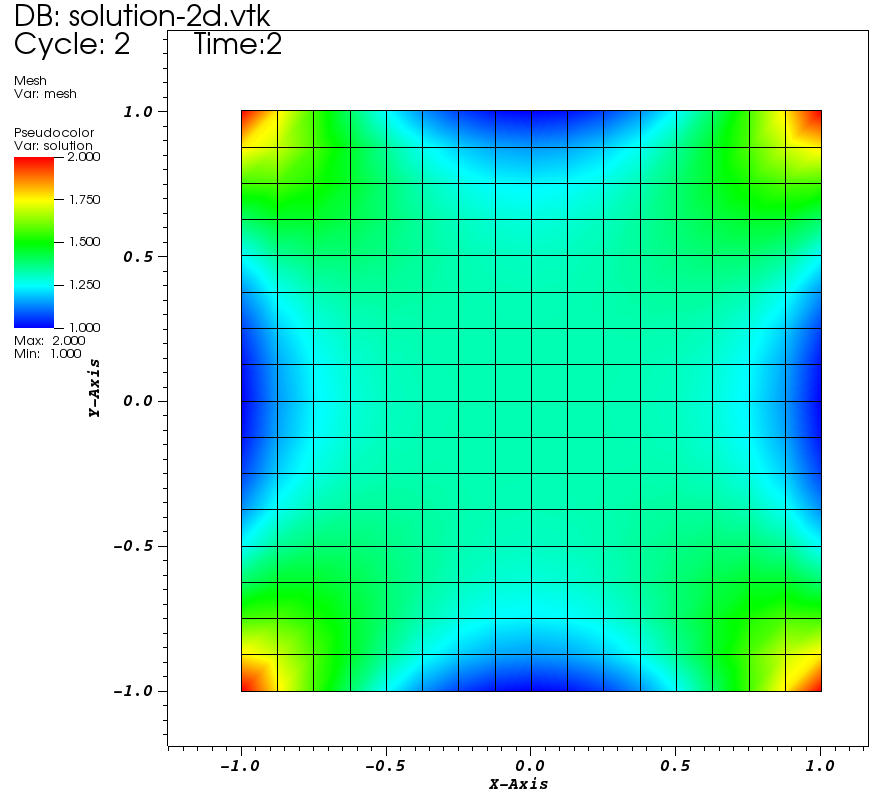
\includegraphics[scale=.7]{Solu2-2d.png}
\end{frame}

\begin{frame}{3D Plot}
	\centering
	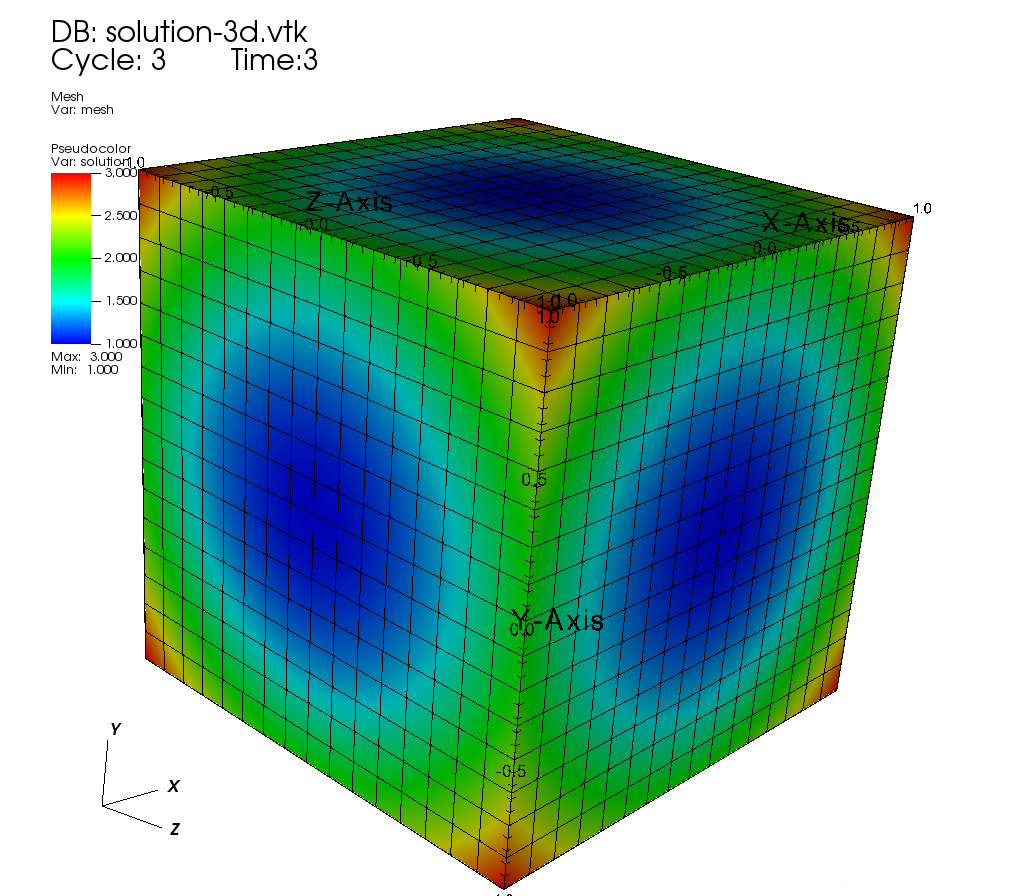
\includegraphics[scale=1]{Solu2-3d.png}
\end{frame}

\begin{frame}{3D Contour Plot}
	\centering
	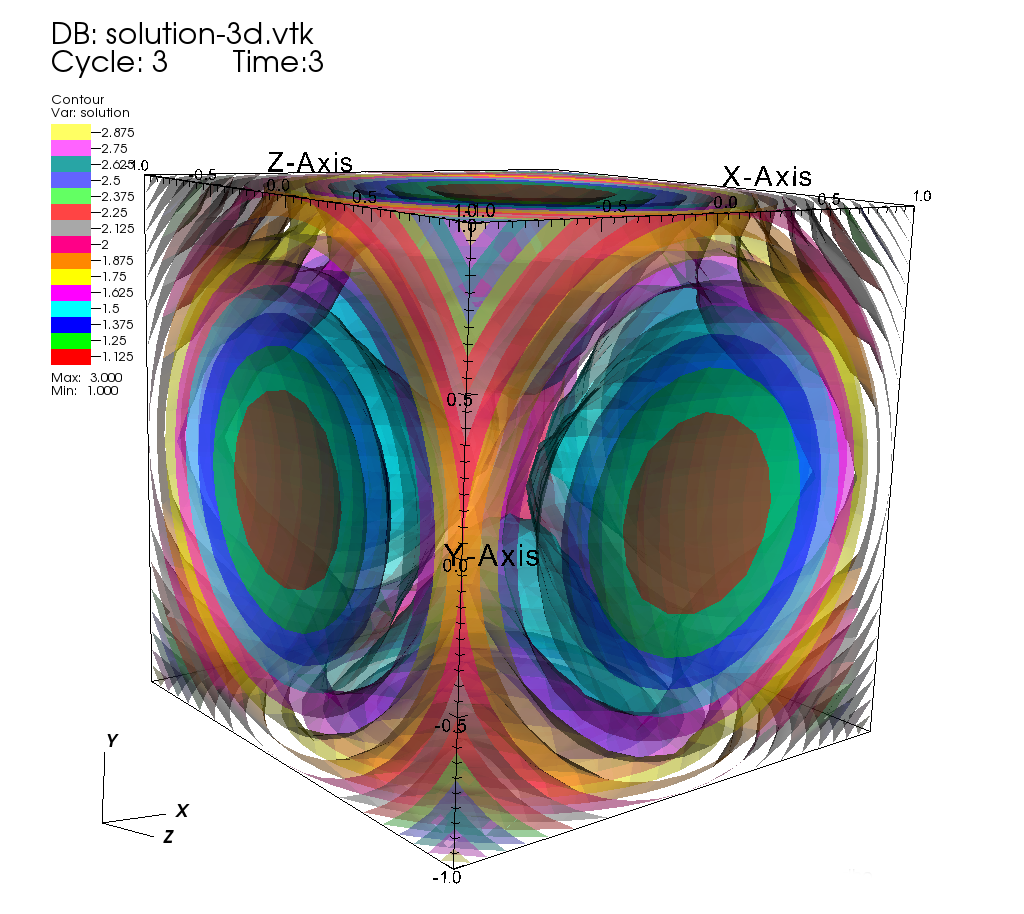
\includegraphics[scale=1]{Solu2-3dcon.png}
\end{frame}

\begin{frame}{Example 3}
	The final PDE solved was Poisson's equation:
	$$
	\begin{cases}
	-\grad \cdot(a(x)\grad u(x)) = 1 &\text{in }\Omega\\
	u = 0 & \text{on }\partial\Omega,
	\end{cases}
	$$
	where $\Omega = [0,1]^2$ and 
	$$
		a(x) = \begin{cases}
		20 & \text{if }\abs{x} < 0.5\\
		1 & \text{otherwise}
		\end{cases}.
	$$ 
	The problem was solved multiple times on increasing global refinements of the mesh.
\end{frame}

\begin{frame}
	\begin{minipage}{.45\paperwidth}
		\centering
		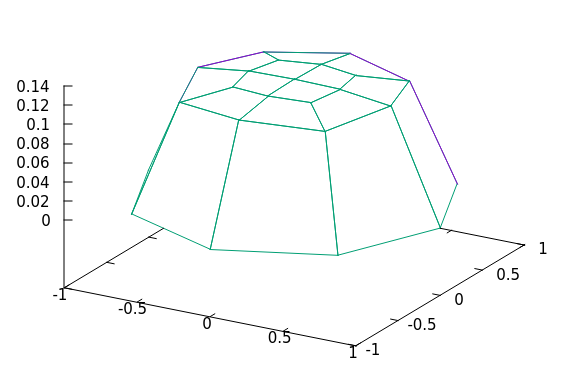
\includegraphics[scale=.5]{Solu3-0.png}
	\end{minipage}%
	\begin{minipage}{.4\paperwidth}
		\centering
		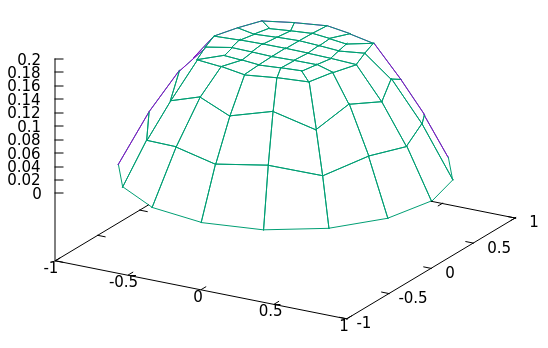
\includegraphics[scale=.5]{Solu3-1.png}
	\end{minipage}
	\begin{minipage}{.45\paperwidth}
		\centering
		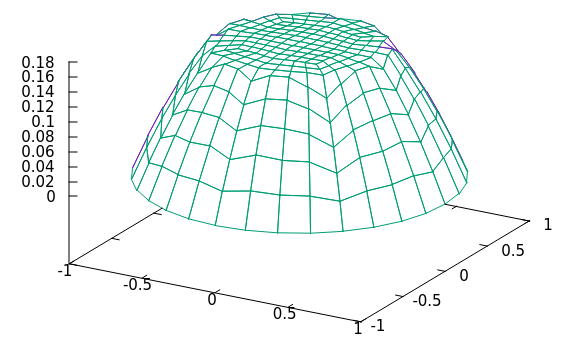
\includegraphics[scale=.5]{Solu3-2.png}
	\end{minipage}%
	\begin{minipage}{.4\paperwidth}
		\centering
		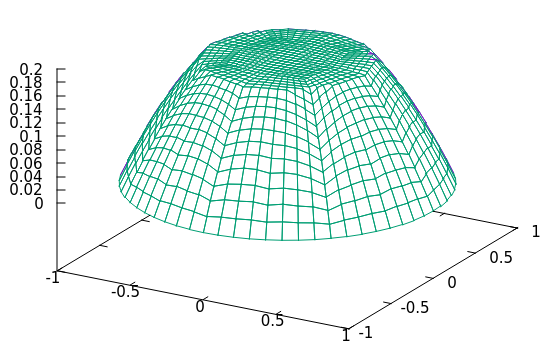
\includegraphics[scale=.5]{Solu3-3.png}
	\end{minipage}
\end{frame}

\begin{frame}{Milestone Updates}
	\begin{itemize}
		\item[1)] Successfully generated and verified input mesh.
		
		\centering
		
\includegraphics[scale=.6]{grid-1.png}
		
		\item[2)] Implement adaptive mesh refinement/coarsening throughout the project, instead of at the end.
		
		\item[3)] Implement and verify the Navier--Stokes solver first, instead of the Cahn--Hilliard solver.
	\end{itemize}
\end{frame}

\begin{frame}{Next Steps}
	\begin{itemize}
		\item[1)] Learn and implement an adaptive local mesh refinement algorithm for stationary problems.
		\vspace{1cm}
		\item[2)] Learn to solve time dependent problems, starting with the heat equation.
		\vspace{1cm}
		\item[3)] Learn to solve the Navier--Stokes problem.
	\end{itemize}
\end{frame}

\end{document}
